% !TEX root = ../main.tex
%
% Copyright 2015
% Jérémy Levallois <jeremy.levallois@gmail.com>
%
% This file and related figures are under Creative Commons CC BY-NC-SA 4.0
% See <https://creativecommons.org/licenses/by-nc-sa/4.0/>
%
\chapter{Conclusions et perspectives}
\label{sec:conclusion}

% \cleanchapterquote{
% %
% My name is Ozymandias, king of kings:\\Look on my works, Ye Mighty, and despair!
% %
% }{Walter \textsc{White}}{Breaking Bad}\footnote{Dans l'épisode, Walter \textsc{White} récite le poème Ozymandias de Percy Bysshe \textsc{Shelley}. Évidemment, aucun lien entre la citation et les travaux présentés ici ne doit être tiré.}
% \cleanchapterquote{We have seen that computer programming is an art, because it
% applies accumulated knowledge to the world, because it requires skill and
% ingenuity, and especially because it produces objects of beauty.}{Jean-Claude
% Vandamme}{Ma vie, mon œuvre.}

Tout au long de cette thèse, nous avons abordé plusieurs approches pour analyser
des contours d'objets digitaux dans l'objectif de les décrire. Nous nous sommes
intéressés dans un premier temps à l'estimation de courbure en dimension 2, puis
de courbure moyenne, courbure gaussienne, courbures
principales, directions principales de courbure et des normales en dimension
3. Ensuite, nous avons proposé un estimateur en dimension 2 et 3 permettant
d'extraire les singularités d'une surface digitale. Ces travaux ont pour but
d'être utilisés dans des algorithmes de plus haut niveau, leurs  propriétés
mathématiques permettant de s'assurer le bon fonctionnement de ceux-ci.

\subsection*{Courbure}
%
Dans le \RefChapitre{sec:estimators}, nous avons décrit le fonctionnement de
l'estimation de la courbure à partir d'intégration volumiques de morceaux de la
surface, puis nous l'avons adapté dans le cadre digital, permettant ainsi une
simplicité de calcul (les intégrales se résumant à dénombrer des points
digitaux) et permettant d'obtenir une validation formelle du comportement
asymptotique de ces estimateurs. La motivation de ce travail était
de proposer des estimateurs digitaux de courbures robustes, avec des preuves de
convergence. De plus, il n'existait aucun estimateur de courbure avec preuves de
convergence en dimension 3.
%
Pour résumer, nous intégrons l'intersection entre une boule et la forme, et
cette quantité nous donne des informations sur la géométrie de la surface, plus
particulièrement sur sa courbure au point de la surface considéré. Ainsi, nous
pouvons extraire la courbure en dimension 2 et la courbure moyenne en dimension
3 à l'aide de l'aire et du volume de l'intersection entre la sphère et la
forme à analyser. Si nous calculons les moments géométriques de cette
intersection, nous pouvons en extraire le tenseur de courbure local de la
surface, et donc les courbures principales, les directions principales de
courbure, la normale, et par extension la courbure gaussienne.
%
Les contributions majeures de ce chapitre sont les preuves de convergence
asymptotique uniforme pour les estimateurs de courbure en dimension 2, de
courbure moyenne et principales en dimension 3. En effet, nous avons montré que
sur des formes convexes à bord $C^3$ à courbure bornée positive, en
paramétrant le rayon de la sphère comme $R = kh^\frac{1}{3}$, nous obtenons des
convergences asymptotiques uniformes en $O(h^\frac{1}{3})$ avec $h$ qui tend
vers $0$.
%
Nous avons également proposé une analyse comparative complète avec des
estimateurs de courbure de la littérature, confirmant expérimentalement la
vitesse de convergence théorique attendue par la preuve. De plus, nous avons
montré que nos estimateurs sont très compétitifs par rapport aux autres, surtout
en restant robuste en présence de bruit et efficace algorithmiquement.


Les perspectives sont multiples pour ces travaux. D'un point de vue pratique,
nous pouvons nous intéresser à faire les calculs dans le domaine de Fourier.
Cela permettrait d’accélérer grandement les temps de calcul pour d'importants rayons
de sphères, car les calculs ne sont plus dépendants de la taille du support mais
linéaires en la taille de l'objet (les convolutions deviennent des
multiplications des transformées de Fourier). Les premiers résultats montrent
une qualité de résultats presque équivalents, avec une vitesse d'exécution
énormément réduite. Cependant, la complexité de ces algorithmes n'est pas
avantageuse : la transformée et la transformée inverse de Fourier de l'objet est
en $O(n^d \log n)$ (le produit est en $O(n^d)$), bien supérieur à notre
algorithme actuel. En pratique, cette version très largement concurrentielle.


Une autre perspective serait le couplage de notre approche avec celles basées
sur les cellules de Voronoï, plus particulièrement les méthodes de \VCMM
\cite{Merigot2009,Merigot2011,Cuel2014DGCI} sur l'analyse de matrice de covariance
non pas de la forme elle même mais du cône normal. Ces approches sont
assez complémentaires avec la nôtre et méritent de s'y intéresser.
%En effet, \VCM a l'avantage de ne pas trop être perturbé sur des objets fins; cependant, des décallages peuvent apparaître sur des arrêtes franches; ce que notre méthode n


De plus, il apparaît que l'erreur de positionnement entre le point digital et le
point sur la surface euclidienne est un terme dominant. Des premiers résultats
lorsque nous approchons mieux la surface sous-jacente montrent une amélioration de
la qualité des résultats, et laissent espérer de meilleures vitesses de
convergence asymptotique.

Enfin, nous devons prendre en compte une
%
\begin{wrapfigure}[8]{r}[0.2cm]{4cm}
	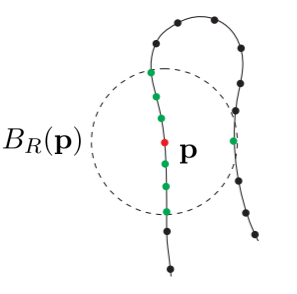
\includegraphics[width=4cm]{images/CriticalRadius}
\end{wrapfigure}
%
considération lors de l'implémentation de ce type
d'estimateurs : puisque nos estimateurs récoltent l'information volumique, il se
peut que de le calcul de l'intégration soit biaisé par l'occultation d'une partie éloignée de l'objet. La figure sur le côté montre cet effet : si le rayon augmente, l'intégration volumique ne sera pas complète. Cela peut être
gênant s'il n'est pas pris en compte et peut ainsi localement fausser les
calculs de courbure. Détecter ces cas devrait améliorer les résultats pour une
forme présentant ce genre de configuration à une échelle donnée.
%
\subsection*{Courbure sans paramètre}
%
Les estimateurs précédents possèdent l'inconvénient que lorsque nous souhaitons récupérer
la valeur de courbure pour un objet particulier, nous devons adapter le rayon de
la sphère en fonction de l'objet. Nous avons alors analysé, dans le
\RefChapitre{sec:estimators}, la géométrie de l'objet digital en amont à
l'aide de segments maximaux afin d'apporter des estimateurs de courbures en
dimension 2 et 3 sans paramètre. Deux versions ont été proposées, une approche «
globale » dont le rayon de la boule d'intégration est lié à la moyenne des
longueurs des segments maximaux de la forme, et une approche « locale » où le
rayon de la sphère est lié aux longueurs des segments maximaux locaux du point
estimé.
%
Nous avons prouvé la convergence asymptotique uniforme de l'estimateur de
courbure en dimension 2 dans son approche « globale » en $O\left(h^\frac{1}{3} \log^2
\left(\frac{1}{3}\right)\right)$ pour des formes convexes à bord $C^3$ à courbure
bornée positive. La preuve de convergence de ces estimateurs en dimension 3
repose sur une supposition non vérifiée à ce jour, qui mériterait d'être étudiée
dans le futur.
%
L'analyse expérimentale a montré que ces deux approches d'estimateurs de
courbure sans paramètre obtiennent des résultats aussi bons que les estimateurs
précédents (en $O(h^\frac{1}{3}$) même en dimension 3, et l'approche « locale »
est très concurrentielle en erreur de norme $l_2$.
%
La motivation principale de ce travail est de palier au manque
d'estimateurs digitaux de courbure en dimension 2 (ou supérieure) sans paramètre
avec des preuves de convergence asymptotiques. De plus, d'un point de vue
pratique, ces estimateurs permettent d'obtenir de bons résultats d'estimation de
courbure sans que l'utilisateur n'ait besoin de choisir de paramètre dépendant de la
forme digitale d'entrée.

Ces estimateurs sans paramètre sont néanmoins moins efficaces en présence de surfaces
bruités. De récents travaux (\cauthors{Kerautret}{Kerautret2012}) proposent
d'estimer le niveau de bruit grâce aux segments maximaux. Nous pouvons
adapter leurs longueurs en fonction du bruit et ainsi augmenter la robustesse de
notre estimation. Cependant, il est peu probable de garantir des preuves de
convergence dans ces conditions; l'application est surtout pratique.
%
\subsection*{Singularités}
%
Enfin, dans le \RefChapitre{sec:applications}, nous avons proposé d'estimer les
singularités sur des objets digitaux. Encore une fois, la principale motivation
de ce travail est de palier au manque d'estimateurs robustes de singularités de
la géométrie digitale. Notre estimateur analyse le comportement de l'estimateur
de courbure défini précédemment à plusieurs rayons de sphère sur le bord de
l'objet, en dimensions 2 et 3. Cette analyse permet de classifier la surface en
trois comportements distincts : des singularités (non-$C^1$), des zones lisses
($C^3$) et des zones à courbure nulle. L'analyse comparative de notre
estimateur avec les méthodes représentatives de la littérature affiche qu'il est compétitif, étant à la fois robuste au bruit, ne
nécessitant pas d'autre paramètre qu'un ensemble de rayons, et classifiant
directement tous les éléments de la surface.


Cet outil est le point d'entrée de plusieurs perspectives intéressantes. Tout
d'abord, les résultats présentés ici sont des résultats bruts. Nous pouvons
facilement coupler notre méthode avec des outils de post-traitement pour
améliorer significativement les défauts encore présents, notamment les artefacts
sur les formes bruités. De plus, des extensions naturelles de ce type
d'estimateur sont le débruitage de forme ou encore la reconstruction de surface,
et notre estimateur pourrait être un très bon point d'entrée.


Ensuite, dans notre estimateur, le rayon maximal de l'ensemble des rayons utilisés pour l'analyse est lié à la distinction de classification de parties
lisse ($C^3$) et de parties à courbure nulle. Si le rayon maximal est trop petit
pour une zone lisse à faible courbure, nous pouvons ne pas détecter la géométrie
locale de la forme (voir le \RefSection{sec:applications:feature:II:kmax}) et
ainsi ne pas la classifier comme une partie lisse. Si nous augmentons ce rayon
maximal, nous pouvons annuler cet effet. Ceci est problématique puisque ça
exige que l'utilisateur analyse la forme avant de choisir les paramètres de
rayons de notre estimateur. Alors, comme pour l'estimation de la courbure,
nous pourrions envisager d'utiliser les segments maximaux afin de permettre de guider l'ensemble de rayons utilisés
pour notre méthode.


Une autre perspective que nous avons un peu abordé dans le
\RefSection{sec:applications:feature:II:transitions} relève du traitement des
zones où une transition de modèle est détectée. Pour résumer, lors de l'analyse des distances aux modèles, certaines zones suivent un modèle avant d'être perturbé par un autre modèle lorsque les rayons diminuent, comme c'est le cas près d'une sigularité par exemple. Actuellement nous prenons
le modèle dominant, mais nous pouvons faire une analyse plus fine de ces
transitions, comme rajouter une dimension à la classification : du rayon $R_a$ à
$R_b$ le point est classifié selon le modèle $A$; du rayon $R_b$ à $R_c$ le
point est classifié selon le modèle $B$, etc. De plus, cela permettrait
également de détecter le changement de statut des points de la surface, comme le
propose \cauthors{Mellado}{Mellado2012} (voir la
\RefFigure{fig:mellado-multiscale}).

%
% \subsection*{Point de vue général}

% Au travers de ces travaux de thèse, j'ai tenté d'apporter ma contribution à la
% communauté de la géométrie digitale.
%
%
% Comme le dit Jean \textsc{Françon} dans la préface de \cite[Coeurjolly2007Book]
%
%
%
% La géométrie digitale possède un ensemble
% d'outils formel
